Sections~\ref{sec:nodefpublished} to~\ref{sec:nodeftrained} use inputs that carry no instruction; from Section~\ref{sec:five} on, every input carries the definition of its task. Every test was written down in the plan of the repository, with the line by which it would be read, before it was run (Section~\ref{sec:protocol}), except where marked. Unless stated, the setting is reduced: T5-base, 10 epochs per task, one seed (42), re-test scoring, and the five tasks of Section~\ref{sec:five} are among the 15 SuperNI development tasks; a test that says ``routes only'' trains nothing.

\subsection{The published methods without their instructions}
\label{sec:nodefpublished}

\paragraph{The published methods without their instructions.} We repeated the five-task run of Section~\ref{sec:five} for InfLoRA and GainLoRA (official code) with the definition of every task replaced by the empty string, in training and testing, so that every input is the same fixed text followed by the instance. The rows of our own method (plain adapters behind \recog{} of Section~\ref{sec:audit}, tested in Section~\ref{sec:recogniser}) are explained in Section~\ref{sec:nodeftrained}.
Line fixed before the run, for each method against its own run with definitions: if the score right after learning is below 60\% of the score with definitions, the method ``could not learn these tasks''; if it learned, it ``holds its answers less well'' when forgetting rises by at least 5 points, or when the changed answers are at least twice as many and at least 60 of 400 higher. Verdict: both learned (score right after learning far above 60\% of that with definitions) and both hold their answers less well: changed answers rise from \AudPubInfloraDefChanged{} to \AudPubInfloraNoDefChanged{} for InfLoRA and from \AudPubGainloraDefChanged{} to \AudPubGainloraNoDefChanged{} for GainLoRA, of \AudPubCompared{} (Table~\ref{tab:noinstpublished}; per task in Table~\ref{tab:noinstpertask}, Appendix~\ref{app:noinstmore}).
The line was set against the three-seed runs with definitions of Section~\ref{sec:five}; the table gives the same seed. Our guess for GainLoRA was 60 to 150 changed answers: \AudPubGainloraNoDefChanged{}.
Caveats written before the run: one seed, five tasks, a small model, a tenth of the published number of epochs; only these two methods were run, a first look in a reduced setting that says nothing about other methods. The two other seeds read the same (Table~\ref{tab:noinstseeds}): over three seeds, changed answers and forgetting stay far above those with definitions (\FiveInfChanged{} and \FiveGainChanged{} answers, \FiveInfFT{} and \FiveGainFT{} points; Section~\ref{sec:five}).

\begin{table}[t]
  \caption{The five tasks of Section~\ref{sec:five}, with the definition of every task in its inputs or none. Score right after learning, final score (Rouge-L) and forgetting; answers changed: of the \AudPubCompared{} test inputs of the first four tasks, those whose answer at the end differs from the answer right after their task was learned (the last task cannot be forgotten). Rows of ours: plain adapters never blocked, with the routes of Section~\ref{sec:audit}, run without definitions only. Last row: every input sent to its own task.}
  \label{tab:noinstpublished}
  \centering
  {\footnotesize\setlength{\tabcolsep}{3pt}\begin{tabular}{p{1.9in}lrrrr}
    \toprule
    Method & Definitions & \shortstack[r]{Score right\\after\\learning $\uparrow$} & \shortstack[r]{Final\\score $\uparrow$} & \shortstack[r]{Forgetting\\(points) $\downarrow$} & \shortstack[r]{Answers\\changed\\of \AudPubCompared{} $\downarrow$} \\
    \midrule
    InfLoRA & with & \AudPubInfloraDefLearned{} & \AudPubInfloraDefAP{} & \AudPubInfloraDefFT{} & \AudPubInfloraDefChanged{} \\
    InfLoRA & none & \AudPubInfloraNoDefLearned{} & \AudPubInfloraNoDefAP{} & \AudPubInfloraNoDefFT{} & \AudPubInfloraNoDefChanged{} \\
    GainLoRA & with & \AudPubGainloraDefLearned{} & \AudPubGainloraDefAP{} & \AudPubGainloraDefFT{} & \AudPubGainloraDefChanged{} \\
    GainLoRA & none & \AudPubGainloraNoDefLearned{} & \AudPubGainloraNoDefAP{} & \AudPubGainloraNoDefFT{} & \AudPubGainloraNoDefChanged{} \\
    \midrule
    \plain{} (all adapters on) & none & \AudOursAllLearned{} & \AudOursAllAP{} & \AudOursAllFT{} & \AudOursAllChanged{} \\
    \recog{} (ours) & none & \AudOursRidgeLearned{} & \AudOursRidgeAP{} & \AudOursRidgeFT{} & \AudOursRidgeChanged{} \\
    \handicap{}, $\nu = 2$ (ours) & none & \AudOursHandicapLearned{} & \AudOursHandicapAP{} & \AudOursHandicapFT{} & \AudOursHandicapChanged{} \\
    every input to its own task (ceiling) & none & \AudOursOwnLearned{} & \AudOursOwnAP{} & \AudOursOwnFT{} & \AudOursOwnChanged{} \\
    \bottomrule
\end{tabular}}

\end{table}

Table~\ref{tab:conflictcount} counts inputs that occur word for word in two tasks, which Proposition~\ref{prop:noinstructionprice} needs. On both standard benchmarks there are none (\AudConfOneShared{} of \AudConfOneInputs{} for the 15 SuperNI tasks, \AudConfTwoShared{} of \AudConfTwoInputs{} for the 15 Long Sequence tasks). The count is a lower limit of the conflict, since tasks can overlap without sharing a text, so alone it shows only that no loss is forced by shared texts. That the loss of the two methods was not forced is shown by the recogniser of Section~\ref{sec:recogniser}, which gives all but \AudRouteFiveRidgeNotOwn{} of the \AudRouteFiveRidgeN{} test inputs of these five tasks to their own task.

\begin{table}[t]
  \caption{Inputs that occur word for word in two or more tasks of a collection (benchmark training and test inputs; instances read from the task files for the fresh batches of Section~\ref{sec:recogniser}). ``Also elsewhere'': inputs that occur in another task of the collection; \%: their share. A count, not a test.}
  \label{tab:conflictcount}
  \centering
  {\footnotesize\setlength{\tabcolsep}{3pt}\begin{tabular}{lrrrr}
    \toprule
    Collection & Tasks & Inputs & \shortstack[r]{Occur also\\in another\\task} & \shortstack[r]{Share,\\\%} \\
    \midrule
    SuperNI, 15 tasks & \AudConfOneTasks{} & \AudConfOneInputs{} & \AudConfOneShared{} & \AudConfOneShare{} \\
    Long Sequence, 15 tasks & \AudConfTwoTasks{} & \AudConfTwoInputs{} & \AudConfTwoShared{} & \AudConfTwoShare{} \\
    fresh batch 1 & \AudConfThreeTasks{} & \AudConfThreeInputs{} & \AudConfThreeShared{} & \AudConfThreeShare{} \\
    fresh batch 2 & \AudConfFourTasks{} & \AudConfFourInputs{} & \AudConfFourShared{} & \AudConfFourShare{} \\
    fresh batch 3 & \AudConfFiveTasks{} & \AudConfFiveInputs{} & \AudConfFiveShared{} & \AudConfFiveShare{} \\
    \bottomrule
\end{tabular}}

\end{table}

\subsection{Recognising the task without an instruction}
\label{sec:recogniser}

\recog{} and its variant \handicap{} (Section~\ref{sec:audit}) read no instruction and block no task. The zone rule of Section~\ref{sec:bound}, tested first in Section~\ref{sec:noinstruction}, left a better frozen feature as the open question. The corrected form of \handicap{} and its setting were chosen after numbers had been seen, and are marked.

\paragraph{The feature.} The zone rule of Section~\ref{sec:noinstruction} (ratio score, level 0.05, the oldest zone wins) was run with a third frozen feature: the mean of the last-layer states of the frozen T5-base encoder, without adapter, over the tokens of the instance. Development data: the 15 SuperNI tasks of order 1, at most 400 training inputs per task, official test inputs.
Line fixed before the run: ``works'' if on average at least 90\% of the test inputs reach their own task and at most 10\% are blocked. Verdict: ``partial'' (Table~\ref{tab:recogniserfeatures}, top): \AudZoneFrozenTOwn{}\% to the own task and \AudZoneFrozenTBlocked{}\% blocked, far better than the sentence encoder and the word vectors, with changed routes within the claim.
The guess, 20 to 35\% blocked, was wrong in the good direction. A likely reason: a sentence encoder keeps what a text is about and discards how it is written, and the way an input is written is most of what separates tasks. The middle of the table shows it for a joint recogniser on sentence-encoder features: 16 numbers describing the shape of the text (length, capitals, digits, punctuation, line breaks, @, \# and web addresses) raise the share at the own task at the end from \AudRecLrMiniEndSuperni{}\% to \AudRecLrShapeEndSuperni{}\% on SuperNI and also on Long Sequence; character n-grams do about as well as the shape numbers.

\begin{table}[t]
  \caption{Features, development data (the benchmark tasks were used to choose among the variants); means over tasks, in \%. Top: the zone rule with three frozen features on the 15 SuperNI tasks (inside own zone; blocked when the task arrives; own task at the end; route changed). Middle: a joint recogniser fitted by logistic regression or by Eq.~\eqref{eq:recogniser} on random cosine features, on the sentence encoder with or without the shape numbers or character n-grams, for SuperNI and Long Sequence; the last pair of columns is $(H{+}1)/(m{+}1)$, where $H$ of the $m$ held-out inputs of a task changed route (Proposition~\ref{prop:audit}), from the held-out inputs. Bottom: the audit of Proposition~\ref{prop:audit} for the chosen variant (logistic regression with shape numbers): $H/m$ and the 95\% bound.}
  \label{tab:recogniserfeatures}
  \centering
  {\footnotesize\setlength{\tabcolsep}{3pt}\begin{tabular}{lrrrr}
    \toprule
    Feature & \shortstack[r]{Inside own\\zone, \%} & \shortstack[r]{Blocked,\\\% $\downarrow$} & \shortstack[r]{Sent to\\own task\\at the end,\\\% $\uparrow$} & \shortstack[r]{Route\\changed,\\\% $\downarrow$} \\
    \midrule
    word vectors & \AudZoneWordVecInside{} & \AudZoneWordVecBlocked{} & \AudZoneWordVecOwn{} & \AudZoneWordVecChanged{} \\
    sentence encoder & \AudZoneSentenceInside{} & \AudZoneSentenceBlocked{} & \AudZoneSentenceOwn{} & \AudZoneSentenceChanged{} \\
    frozen T5-base states & \AudZoneFrozenTInside{} & \AudZoneFrozenTBlocked{} & \AudZoneFrozenTOwn{} & \AudZoneFrozenTChanged{} \\
    \bottomrule
\end{tabular}}
\par\medskip
{\footnotesize\setlength{\tabcolsep}{1.8pt}\begin{tabular}{lrrrrrr}
    \toprule
    & \multicolumn{2}{c}{\shortstack{Sent to own task\\at the end, \% $\uparrow$}} & \multicolumn{2}{c}{\shortstack{Route changed,\\\% $\downarrow$}} & \multicolumn{2}{c}{\shortstack{Audit\\$(H{+}1)/(m{+}1)$, \%}} \\
    \cmidrule(lr){2-3}\cmidrule(lr){4-5}\cmidrule(l){6-7}
    Recogniser, feature & SuperNI & Long & SuperNI & Long & SuperNI & Long \\
    \midrule
    logistic reg., sentence enc., $C=$\AudRecLrMiniParam{} & \AudRecLrMiniEndSuperni{} & \AudRecLrMiniEndLong{} & \AudRecLrMiniChangedSuperni{} & \AudRecLrMiniChangedLong{} & \AudRecLrMiniAuditLineSuperni{} & \AudRecLrMiniAuditLineLong{} \\
    \textbf{\quad + shape numbers, $C=$\AudRecLrShapeParam{}} & \textbf{\AudRecLrShapeEndSuperni{}} & \textbf{\AudRecLrShapeEndLong{}} & \textbf{\AudRecLrShapeChangedSuperni{}} & \textbf{\AudRecLrShapeChangedLong{}} & \textbf{\AudRecLrShapeAuditLineSuperni{}} & \textbf{\AudRecLrShapeAuditLineLong{}} \\
    \quad + character n-grams, $C=$\AudRecLrCharParam{} & \AudRecLrCharEndSuperni{} & \AudRecLrCharEndLong{} & \AudRecLrCharChangedSuperni{} & \AudRecLrCharChangedLong{} & \AudRecLrCharAuditLineSuperni{} & \AudRecLrCharAuditLineLong{} \\
    cosine features, sentence enc., $\lambda=$\AudRecCosMiniParam{} & \AudRecCosMiniEndSuperni{} & \AudRecCosMiniEndLong{} & \AudRecCosMiniChangedSuperni{} & \AudRecCosMiniChangedLong{} & \AudRecCosMiniAuditLineSuperni{} & \AudRecCosMiniAuditLineLong{} \\
    \quad + shape numbers, $\lambda=$\AudRecCosShapeParam{} & \AudRecCosShapeEndSuperni{} & \AudRecCosShapeEndLong{} & \AudRecCosShapeChangedSuperni{} & \AudRecCosShapeChangedLong{} & \AudRecCosShapeAuditLineSuperni{} & \AudRecCosShapeAuditLineLong{} \\
    \bottomrule
\end{tabular}}
\par\medskip
{\footnotesize\setlength{\tabcolsep}{3pt}\begin{tabular}{lrrrr}
    \toprule
    & \multicolumn{2}{c}{Audit $H/m$, \%} & \multicolumn{2}{c}{95\% bound, \%} \\
    \cmidrule(lr){2-3}\cmidrule(l){4-5}
    Chosen variant & SuperNI & Long & SuperNI & Long \\
    \midrule
    logistic reg. + shape numbers, $C=$\AudRecLrShapeParam{} & \AudRecChosenAuditEstSuperni{} & \AudRecChosenAuditEstLong{} & \AudRecChosenAuditBoundSuperni{} & \AudRecChosenAuditBoundLong{} \\
    \bottomrule
\end{tabular}}

\end{table}

\paragraph{Rules that block nothing.} Development data: the 15 SuperNI tasks, at most 400 training inputs per task, 200 of them held out (half for tasks with fewer than 400), official test inputs; the rules run on the frozen T5-base states, standardised with the statistics of 2{,}000 instances of other SuperNI tasks (the pool of Section~\ref{sec:protocol}, not $\mathcal{B}$).
Rule written before the run: among the variants with at most 3\% changed routes, take the highest share of test inputs at their own task after the last task; ties go to the ridge form, which stores no input. Verdict: it chose \recog{} with the smallest of three penalties (``ridge $1\times$'': in the code a penalty equal to the feature dimension, 768, on sums with total weight 200 per task; in Eq.~\eqref{eq:recogniser}, $\varepsilon = 768/200 = 3.84$), tied with the logistic regression (Table~\ref{tab:recogniserdev}).
It gives \AudDevLLamOneEnd{}\% of the test inputs to their own task after the last task, with \AudDevLLamOneChanged{}\% of the routes changed; the audit of Proposition~\ref{prop:audit} has a 95\% bound of \AudDevLLamOneAuditBound{}\%. The weights are the same for every order of arrival, up to rounding (checked with the order reversed); on the second official order and on five random orders the changed routes run from \AudOrdRandTwoLChanged{}\% to \AudOrdTwoLChanged{}\% (Table~\ref{tab:recogniserorders}, Appendix~\ref{app:noinstmore}).
The guess, 95 to 99\%, held; the guess of 1 to 3\% changed routes was too high (\AudDevLLamOneChanged{}\%). Weak tasks: the tweet task (sentiment140) falls from \AudPtFourteenArrive{}\% to \AudPtFourteenEnd{}\% when the emotion task arrives (\AudPtFourteenC{} of its \AudPtFourteenM{} held-out inputs change route, and the audit shows it) and the dialogue task (multi-woz) ends at \AudPtSevenEnd{}\%; all others end at 99 to 100\% (Table~\ref{tab:recogniserpertask}, Appendix~\ref{app:noinstmore}).

\begin{table}[t]
  \caption{Rules that block nothing, development data: the 15 SuperNI tasks of order 1, frozen T5-base states, means over tasks, in \%. Own task at arrival and after the last task; route changed after the task arrived; audit $H/m$ and 95\% bound (Proposition~\ref{prop:audit}, held-out inputs); bound in advance (Theorem~\ref{thm:handicap} for \handicap{}; for the zone rule the line of the zone paragraph, not a theorem). $C$: inverse penalty of the logistic regression; ridge $1\times$, $10\times$, $100\times$: penalty of Eq.~\eqref{eq:recogniser} in multiples of the smallest; $r$: a new zone may hold at most $r-1$ held-out inputs of an older task. Bold: the variants used later. The last three rows are the first form of \handicap{}, without the floor at zero in Eq.~\eqref{eq:handicap}. The rows were compared on these tasks: development numbers.}
  \label{tab:recogniserdev}
  \centering
  {\scriptsize\setlength{\tabcolsep}{2.5pt}\begin{tabular}{p{1.6in}rrrrrr}
    \toprule
    Rule & \shortstack[r]{Sent to\\own task\\at arrival,\\\% $\uparrow$} & \shortstack[r]{Sent to\\own task\\at the end,\\\% $\uparrow$} & \shortstack[r]{Route\\changed,\\\% $\downarrow$} & \shortstack[r]{Audit\\$H/m$, \%} & \shortstack[r]{95\% bound,\\\%} & \shortstack[r]{Bound in\\advance, \%} \\
    \midrule
    \recog{} with logistic regression ($C = 1$) & \AudDevJCOneArrive{} & \AudDevJCOneEnd{} & \AudDevJCOneChanged{} & \AudDevJCOneAuditEst{} & \AudDevJCOneAuditBound{} & -- \\
    \textbf{\recog{}, ridge $1\times$} & \textbf{\AudDevLLamOneArrive{}} & \textbf{\AudDevLLamOneEnd{}} & \textbf{\AudDevLLamOneChanged{}} & \textbf{\AudDevLLamOneAuditEst{}} & \textbf{\AudDevLLamOneAuditBound{}} & \textbf{--} \\
    \recog{}, ridge $10\times$ & \AudDevLLamTenArrive{} & \AudDevLLamTenEnd{} & \AudDevLLamTenChanged{} & \AudDevLLamTenAuditEst{} & \AudDevLLamTenAuditBound{} & -- \\
    \recog{}, ridge $100\times$ & \AudDevLLamHundredArrive{} & \AudDevLLamHundredEnd{} & \AudDevLLamHundredChanged{} & \AudDevLLamHundredAuditEst{} & \AudDevLLamHundredAuditBound{} & -- \\
    zones, newest wins, $r = 1$ & \AudDevClaimsROneArrive{} & \AudDevClaimsROneEnd{} & \AudDevClaimsROneChanged{} & -- & -- & \AudDevClaimsROneBound{} \\
    \handicap{}, $\nu = 0$ & \AudDevHPrimeTZeroArrive{} & \AudDevHPrimeTZeroEnd{} & \AudDevHPrimeTZeroChanged{} & -- & -- & \AudDevHPrimeTZeroBound{} \\
    \handicap{}, $\nu = 1$ & \AudDevHPrimeTOneArrive{} & \AudDevHPrimeTOneEnd{} & \AudDevHPrimeTOneChanged{} & -- & -- & \AudDevHPrimeTOneBound{} \\
    \textbf{\handicap{}, $\nu = 2$} & \textbf{\AudDevHPrimeTTwoArrive{}} & \textbf{\AudDevHPrimeTTwoEnd{}} & \textbf{\AudDevHPrimeTTwoChanged{}} & \textbf{--} & \textbf{--} & \textbf{\AudDevHPrimeTTwoBound{}} \\
    \handicap{}, $\nu = 5$ & \AudDevHPrimeTFiveArrive{} & \AudDevHPrimeTFiveEnd{} & \AudDevHPrimeTFiveChanged{} & -- & -- & \AudDevHPrimeTFiveBound{} \\
    \handicap{} without protection ($\nu = \infty$) & \AudDevHPrimeTNoneArrive{} & \AudDevHPrimeTNoneEnd{} & \AudDevHPrimeTNoneChanged{} & -- & -- & -- \\
    \midrule
    \handicap{} without the floor (first form), $\nu = 0$ & \AudDevHTZeroArrive{} & \AudDevHTZeroEnd{} & \AudDevHTZeroChanged{} & -- & -- & \AudDevHTZeroBound{} \\
    \handicap{} without the floor (first form), $\nu = 1$ & \AudDevHTOneArrive{} & \AudDevHTOneEnd{} & \AudDevHTOneChanged{} & -- & -- & \AudDevHTOneBound{} \\
    \handicap{} without the floor (first form), $\nu = 2$ & \AudDevHTTwoArrive{} & \AudDevHTTwoEnd{} & \AudDevHTTwoChanged{} & -- & -- & \AudDevHTTwoBound{} \\
    \bottomrule
\end{tabular}}

\end{table}

\paragraph{\handicap{}, and a flaw in its first form.} \handicap{} (Eq.~\eqref{eq:handicap}) puts a bound known in advance on the same joint recogniser. As first written, the threshold $\eta_k$ had no floor at zero: when no held-out input of an older task lies near the newcomer, it is negative and the newcomer takes inputs that even the joint recogniser gives to an older task. For $\nu = 2$ the first form changed more routes than no protection: \AudDevHTTwoChanged{}\% against \AudDevHPrimeTNoneChanged{}\% (also for $\nu = 1$). The guess for $\nu = 0$, 97 to 99\% at the own task, was wrong: \AudDevHTZeroEnd{}\%.
The floor at zero is the correction. It was made after seeing these numbers, on the same 15 tasks, so the numbers of the corrected rule are development numbers; the proof is unchanged. With the floor, the share at the own task at the end is \AudDevHPrimeTZeroEnd{}\% for $\nu = 0$ and \AudDevHPrimeTTwoEnd{}\% for $\nu = 2$, close to no protection, and the changed routes fall to \AudDevHPrimeTTwoChanged{}\% (Table~\ref{tab:recogniserdev}).
We then chose $\nu = 2$, the smallest value within 0.2 points of the best at the end ($\nu = 5$: \AudDevHPrimeTFiveEnd{}\%). With $\nu = 0$ quoref takes only about a third of its own inputs, because one held-out input of the news task sets the threshold (Remark~\ref{rem:auditlimits}(ii)). For $\nu = 2$ the bound in advance averages \AudDevHPrimeTTwoBound{}\%, far above what was measured: it is loose, because most later tasks take nothing from most older ones, which it cannot know.

\paragraph{Zones can do it too, with the right feature.} Four zone shapes were compared on the sentence encoder, before the joint recogniser was chosen, under one rule: the newest zone wins, and no held-out input of an older task may lie inside a new zone, so no task is blocked (15 SuperNI tasks, development data; the Long Sequence part of the grid was not computed).
The rule written before the grid chose one boundary per older task with the shape numbers (weight \AudShapePairShapeWeight{}): \AudShapePairShapeEnd{}\% at the end, \AudShapePairShapeChanged{}\% of the routes changed, against a line of \AudShapePairShapeBound{}\%. The line is the share of a task's test inputs outside its own zone at arrival plus $r/(m+1)$ for every later task; it follows from the rank argument of Theorem~\ref{thm:handicap}, but is used as a line fixed in advance, not stated as a theorem.
The shape matters less than the feature: with the shape numbers three shapes reach \AudShapeOvrShapeEnd{}\% to \AudShapePairShapeEnd{}\%, the balls \AudShapePairKnnShapeEnd{}\%, and without the numbers the same three are lower (Table~\ref{tab:shapesgrid}). No guess was written for the shapes.

\begin{table}[t]
  \caption{Four zone shapes, development data: the 15 SuperNI tasks, sentence encoder alone or with the 16 shape numbers (best weight tried). Rows: one flat boundary against everything older, one per older task, balls, boundaries curved by random cosine features. Means over tasks, in \%: own task after the last task; route changed. Bold: the variant chosen by the rule written before the grid.}
  \label{tab:shapesgrid}
  \centering
  {\footnotesize\setlength{\tabcolsep}{3pt}\begin{tabular}{lrrrrr}
    \toprule
    & \multicolumn{2}{c}{Sentence encoder} & \multicolumn{3}{c}{+ shape numbers} \\
    \cmidrule(lr){2-3}\cmidrule(l){4-6}
    Boundary & \shortstack[r]{Sent to\\own task\\at the end,\\\% $\uparrow$} & \shortstack[r]{Route\\changed,\\\% $\downarrow$} & \shortstack[r]{Sent to\\own task\\at the end,\\\% $\uparrow$} & \shortstack[r]{Route\\changed,\\\% $\downarrow$} & weight \\
    \midrule
    one boundary against everything & \AudShapeOvrMiniEnd{} & \AudShapeOvrMiniChanged{} & \AudShapeOvrShapeEnd{} & \AudShapeOvrShapeChanged{} & \AudShapeOvrShapeWeight{} \\
    one boundary per older task & \AudShapePairMiniEnd{} & \AudShapePairMiniChanged{} & \textbf{\AudShapePairShapeEnd{}} & \textbf{\AudShapePairShapeChanged{}} & \textbf{\AudShapePairShapeWeight{}} \\
    balls around the task's inputs & \AudShapePairKnnMiniEnd{} & \AudShapePairKnnMiniChanged{} & \AudShapePairKnnShapeEnd{} & \AudShapePairKnnShapeChanged{} & \AudShapePairKnnShapeWeight{} \\
    curved boundaries & \AudShapePairRffMiniEnd{} & \AudShapePairRffMiniChanged{} & \AudShapePairRffShapeEnd{} & \AudShapePairRffShapeChanged{} & \AudShapePairRffShapeWeight{} \\
    \bottomrule
\end{tabular}}

\end{table}

\paragraph{Fresh tasks.} Each rule was chosen on the 15 benchmark tasks and read once on a batch of 30 fresh tasks that no earlier test had used (drawn at random from a collection of real tasks, instances only; at least 1{,}000 instances each, the last 200 as test inputs, training and held-out inputs from a random part of the first 800).
Lines fixed before: a rule ``works'' if on average at least 85\% of the test inputs go to their own task, both at arrival and after the last task, ``does not'' below 70\%, else ``partial''; for the oldest-zone-wins rule also at most 15\% blocked, ``does not'' above 30\%; a guarantee is ``met'' if the average changed share is at most the average bound (for the audit, the average $(H{+}1)/(m{+}1)$) plus two standard errors.
Verdicts (Table~\ref{tab:recogniserfresh}): first batch, both zone rules on the sentence encoder did not work (oldest zone wins: \AudShapeFreshFirstOldestEnd{}\% at the end with \AudShapeFreshFirstOldestBlocked{}\% blocked, ``\AudShapeFreshFirstOldestUse{}''; newest zone wins: \AudShapeFreshFirstNewestEnd{}\%, ``\AudShapeFreshFirstNewestUse{}''). Second batch, zone rule with one boundary per older task and shape numbers: \AudShapeFreshSecondEnd{}\% at the end, changed routes within its line of \AudShapeFreshSecondBound{}\%, ``\AudShapeFreshSecondUse{}'', guarantee ``\AudShapeFreshSecondGuarantee{}''. Third batch, joint recogniser (logistic regression, sentence encoder, shape numbers): \AudFreshThirdEnd{}\% at the end, ``\AudFreshThirdUse{}'', audit line $(H{+}1)/(m{+}1)$ \AudFreshThirdAuditLine{}\%, audit ``\AudFreshThirdCert{}''. Fourth batch, \recog{} on the frozen model's states, the rule used for trained answers: \AudFreshFourthLEnd{}\% at the end, ``\AudFreshFourthUse{}'', audit line \AudFreshFourthLAuditLine{}\%, audit ``\AudFreshFourthCert{}''; the changed routes and audit bounds are in the table. The guess, 80 to 90\%, was too low.
On the fourth batch \handicap{} ($\nu = 2$), reported by a line fixed before (within 2 points of \recog{} at the end), reaches \AudFreshFourthHEnd{}\% and changes fewer routes. The batches differ, so the rows do not compare the rules.

\begin{table}[t]
  \caption{Fresh tasks: each rule read once on a batch of 30 tasks that nothing had used. Means over the 30 tasks, in \%: own task at arrival and after the last task; routes changed; audit $H/m$ and 95\% bound where the rule has an audit. Verdict: use / guarantee by the lines in the text. Last column: number of tasks below 70\% own task.}
  \label{tab:recogniserfresh}
  \centering
  {\scriptsize\setlength{\tabcolsep}{2pt}\begin{tabular}{p{0.95in}rrrrrcr}
    \toprule
    Fresh tasks & \shortstack[r]{Sent to\\own task\\at arrival,\\\% $\uparrow$} & \shortstack[r]{Sent to\\own task\\at the end,\\\% $\uparrow$} & \shortstack[r]{Route\\changed,\\\% $\downarrow$} & \shortstack[r]{Audit\\$H/m$, \%} & \shortstack[r]{95\% bound,\\\%} & Verdict & \shortstack[r]{Tasks below\\70\% $\downarrow$} \\
    \midrule
    first batch: zones, oldest wins, sentence encoder & -- & \AudShapeFreshFirstOldestEnd{} & \AudShapeFreshFirstOldestChanged{} & -- & -- & \AudShapeFreshFirstOldestUse{} / \AudShapeFreshFirstOldestClaim{} & -- \\
    first batch: zones, newest wins, sentence encoder & \AudShapeFreshFirstNewestArrive{} & \AudShapeFreshFirstNewestEnd{} & \AudShapeFreshFirstNewestChanged{} & -- & -- & \AudShapeFreshFirstNewestUse{} / \AudShapeFreshFirstNewestGuarantee{} & -- \\
    second batch: zones, newest wins, one boundary per older task, sentence encoder + shape numbers & \AudShapeFreshSecondArrive{} & \AudShapeFreshSecondEnd{} & \AudShapeFreshSecondChanged{} & -- & -- & \AudShapeFreshSecondUse{} / \AudShapeFreshSecondGuarantee{} & -- \\
    third batch: sentence enc. + shape numbers, logistic reg. & \AudFreshThirdArrive{} & \AudFreshThirdEnd{} & \AudFreshThirdChanged{} & \AudFreshThirdAuditEst{} & \AudFreshThirdAuditBound{} & \AudFreshThirdUse{} / \AudFreshThirdCert{} & \AudFreshThirdLow{} \\
    fourth batch: frozen T5-base states, \recog{} & \AudFreshFourthLArrive{} & \AudFreshFourthLEnd{} & \AudFreshFourthLChanged{} & \AudFreshFourthAuditEst{} & \AudFreshFourthAuditBound{} & \AudFreshFourthUse{} / \AudFreshFourthCert{} & \AudFreshFourthLow{} \\
    fourth batch: frozen T5-base states, \handicap{}, $\nu = 2$ & \AudFreshFourthHArrive{} & \AudFreshFourthHEnd{} & \AudFreshFourthHChanged{} & -- & -- & -- & -- \\
    \bottomrule
\end{tabular}}

\end{table}

The failure belongs to the third batch and returns in the fourth. Two tasks of the third batch are built on the same dataset (answers for a question, and a question for an answer); Table~\ref{tab:conflictcount} shows \AudConfFiveShared{} inputs of \AudConfFiveInputs{} (\AudConfFiveShare{}\%) that occur in two tasks, all in this pair, and none in the first two batches (the fourth was not counted). Each of the two gets about half of its own inputs (\AudFreshThirdPairLow{}\% and \AudFreshThirdPairHigh{}\%). This is the conflict of Proposition~\ref{prop:noinstructionprice} in data: \AudConfPairShare{}\% of the inputs of each occur in the other, and on those no method without instructions can do better than split them. The rest of the loss is not forced by this count, though their other inputs are texts of the same kind; the other tasks of the batch are unaffected.
The fourth batch has a pair on the same reading passages (its shared texts were not counted): under \recog{} the older task falls to about half of its inputs when the newer one arrives, and its audit shows it; under \handicap{} the older keeps its routes and the newer is kept out. The price moves; it does not go away.
Caveat from the independent check: the test inputs are the last 200 instances of a task file and the held-out inputs a random part of the first 800. If a file is ordered the two are not the same kind of draw, so the statements about change rest on an assumption not ensured by construction; the shares at the own task do not depend on it.

\paragraph{The second benchmark, and many tasks.} Frozen states were computed on a GPU (they are slow on a CPU); routes only. These tasks had been used to compare features for an earlier variant; \recog{} and its one setting had been fixed on SuperNI before it was read on them.
Line fixed before the run: \recog{} ``works on the second benchmark'' if at least 90\% of all official test inputs of the 15 Long Sequence tasks go to their own task after the last task, ``does not'' below 75\%. Verdict: ``works'', audit ``met'': \AudScaleLongThreeEnd{}\% for both official orders (Table~\ref{tab:recogniserscale}). The guess, 94 to 98\%, held. The weak tasks are two of three entailment tasks: mnli falls to \AudScaleLongMnliEnd{}\% when rte arrives (\AudScaleLongMnliC{} of \AudScaleLongMnliM{} held-out inputs change route) and rte gets \AudScaleLongRteEnd{}\%; under \handicap{} mnli keeps its inputs and rte takes only \AudScaleLongRteHEnd{}\% (Table~\ref{tab:recogniserlongpertask}, Appendix~\ref{app:noinstmore}).
Many tasks, on the three fresh batches that earlier tests had used, so a description and not a verdict: with 30, 60, 90 fresh tasks and all 120 tasks together, the share of \recog{} at the own task falls from \AudScaleFreshThirtyEnd{}\% to \AudScaleAllHundredTwentyEnd{}\% (Figure~\ref{fig:recogniserscale}); at 120 tasks the changed routes are \AudScaleAllHundredTwentyChanged{}\% and the audit follows (bound \AudScaleAllHundredTwentyAuditBound{}\%). \handicap{} changes about 1\% at every size and gives two to three points fewer at the own task (\AudScaleAllHundredTwentyHEnd{}\%); its bound in advance says nothing at this size. The guess for 120 tasks, 90 to 95\%, held.
On the pair built on the same texts, \recog{} takes the older task from \AudScalePairOlderLArrival{}\% to \AudScalePairOlderLEnd{}\% and gives the newer \AudScalePairNewerLEnd{}\%; \handicap{} keeps the older at \AudScalePairOlderHEnd{}\% and gives the newer \AudScalePairNewerHEnd{}\%.
Two checks ran inside the job: the 15 SuperNI tasks reproduce the CPU numbers, and all \AudScaleFingerprintMatch{} of \AudScaleFingerprintTotal{} downloaded task files hold the same texts as on the CPU. A second version of the fresh sequences with one random split of all instances, made because of the caveat above, moved the shares by \AudScaleSplitMaxDiffEnd{} points or less.

\begin{table}[t]
  \caption{\recog{} and \handicap{} ($\nu = 2$) on the two benchmarks and on growing collections of tasks (frozen T5-base states on a GPU, routes only); means over tasks, in \%. Long Sequence rows: all official test inputs, read against a line fixed in advance; fresh-task rows: batches earlier tests had seen, a description. Audit $H/m$ and 95\% bound: Proposition~\ref{prop:audit}.}
  \label{tab:recogniserscale}
  \centering
  {\scriptsize\setlength{\tabcolsep}{2.5pt}\begin{tabular}{p{0.85in}rrrrrrrr}
    \toprule
    & & \multicolumn{5}{c}{\recog{}} & \multicolumn{2}{c}{\handicap{}, $\nu = 2$} \\
    \cmidrule(lr){3-7}\cmidrule(l){8-9}
    Sequence & Tasks & \shortstack[r]{Sent\\to own\\task\\at\\arrival,\\\% $\uparrow$} & \shortstack[r]{Sent\\to own\\task\\at the\\end,\\\% $\uparrow$} & \shortstack[r]{Route\\changed,\\\% $\downarrow$} & \shortstack[r]{Audit\\$H/m$, \%} & \shortstack[r]{95\% bound,\\\%} & \shortstack[r]{Sent\\to own\\task\\at the\\end,\\\% $\uparrow$} & \shortstack[r]{Route\\changed,\\\% $\downarrow$} \\
    \midrule
    SuperNI order 1 & \AudScaleSuperniOneTasks{} & \AudScaleSuperniOneArrive{} & \AudScaleSuperniOneEnd{} & \AudScaleSuperniOneChanged{} & \AudScaleSuperniOneAuditEst{} & \AudScaleSuperniOneAuditBound{} & \AudScaleSuperniOneHEnd{} & \AudScaleSuperniOneHChanged{} \\
    SuperNI order 2 & \AudScaleSuperniTwoTasks{} & \AudScaleSuperniTwoArrive{} & \AudScaleSuperniTwoEnd{} & \AudScaleSuperniTwoChanged{} & \AudScaleSuperniTwoAuditEst{} & \AudScaleSuperniTwoAuditBound{} & \AudScaleSuperniTwoHEnd{} & \AudScaleSuperniTwoHChanged{} \\
    Long Sequence order 3 & \AudScaleLongThreeTasks{} & \AudScaleLongThreeArrive{} & \AudScaleLongThreeEnd{} & \AudScaleLongThreeChanged{} & \AudScaleLongThreeAuditEst{} & \AudScaleLongThreeAuditBound{} & \AudScaleLongThreeHEnd{} & \AudScaleLongThreeHChanged{} \\
    Long Sequence order 4 & \AudScaleLongFourTasks{} & \AudScaleLongFourArrive{} & \AudScaleLongFourEnd{} & \AudScaleLongFourChanged{} & \AudScaleLongFourAuditEst{} & \AudScaleLongFourAuditBound{} & \AudScaleLongFourHEnd{} & \AudScaleLongFourHChanged{} \\
    fresh batch 1 & \AudScaleFreshThirtyTasks{} & \AudScaleFreshThirtyArrive{} & \AudScaleFreshThirtyEnd{} & \AudScaleFreshThirtyChanged{} & \AudScaleFreshThirtyAuditEst{} & \AudScaleFreshThirtyAuditBound{} & \AudScaleFreshThirtyHEnd{} & \AudScaleFreshThirtyHChanged{} \\
    fresh batches 1+2 & \AudScaleFreshSixtyTasks{} & \AudScaleFreshSixtyArrive{} & \AudScaleFreshSixtyEnd{} & \AudScaleFreshSixtyChanged{} & \AudScaleFreshSixtyAuditEst{} & \AudScaleFreshSixtyAuditBound{} & \AudScaleFreshSixtyHEnd{} & \AudScaleFreshSixtyHChanged{} \\
    fresh batches 1+2+3 & \AudScaleFreshNinetyTasks{} & \AudScaleFreshNinetyArrive{} & \AudScaleFreshNinetyEnd{} & \AudScaleFreshNinetyChanged{} & \AudScaleFreshNinetyAuditEst{} & \AudScaleFreshNinetyAuditBound{} & \AudScaleFreshNinetyHEnd{} & \AudScaleFreshNinetyHChanged{} \\
    all & \AudScaleAllHundredTwentyTasks{} & \AudScaleAllHundredTwentyArrive{} & \AudScaleAllHundredTwentyEnd{} & \AudScaleAllHundredTwentyChanged{} & \AudScaleAllHundredTwentyAuditEst{} & \AudScaleAllHundredTwentyAuditBound{} & \AudScaleAllHundredTwentyHEnd{} & \AudScaleAllHundredTwentyHChanged{} \\
    \bottomrule
\end{tabular}}

\end{table}

\begin{figure}[t]
  \centering
  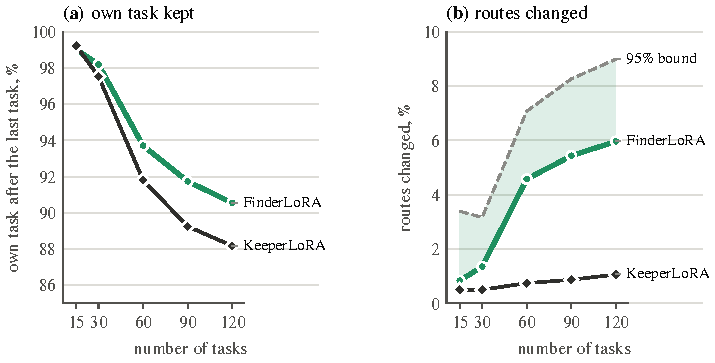
\includegraphics[width=\linewidth]{figures/recogniser_scale}
  \caption{Many tasks, routes only. Left: share of test inputs at their own task after the last task. Right: share of routes changed, with the 95\% bound of the audit for \recog{}. The point at 15 tasks is SuperNI; the others are 30, 60, 90 fresh tasks and all 120 together.}
  \label{fig:recogniserscale}
\end{figure}

\subsection{Trained answers without instructions}
\label{sec:nodeftrained}

\paragraph{Trained answers on a small model.} The stand-alone code (\texttt{t5-small}, the five tasks, no definition, one seed, CPU) was run with the routes of \recog{} on the frozen states of that small model, by the lines of the earlier pilot (Section~\ref{sec:noinstruction}): at most 20 of 200 answers changed and forgetting at most 3 points while more than 100 change with all adapters on; score right after learning at least 90\% of that with all adapters on; at least 80\% of test inputs at their own task. Verdict: ``works''. With all adapters on, \AudSmallAllChanged{} of \AudSmallAllCompared{} answers changed and the score fell from \AudSmallAllLearned{} to \AudSmallAllAP{}; with the routes, \AudSmallRidgeChanged{} of \AudSmallRidgeCompared{} changed, forgetting was \AudSmallRidgeFT{}, the score went from \AudSmallRidgeLearned{} to \AudSmallRidgeAP{}, and 97.2\% reached their own task. Two of the five tasks are learned poorly by this model under either rule, so they add little; the check was planned before the GPU run below and finished after it.

\paragraph{Trained answers: our method against the published methods.} Plain adapters that are never blocked, on a GPU: while task $t$ is learned, adapters $1$ to $t$ are on for all its inputs, and at test time an input is answered by the adapters that existed when the task it is routed to was learned. The routes of \recog{} and \handicap{} ($\nu = 2$) on the frozen T5-base states of the instance were written to the repository before the run (Table~\ref{tab:routesgpu}).
Line fixed before the run: ``beats the published methods in this setting'' if the final score is at least 2 points above the better published method without definitions, forgetting is below 2 points, and at most 32 of the \AudOursRidgeCompared{} compared answers change (a quarter of what GainLoRA changes); ``does not'' if the final score is below that of the better published method or at least \AudPubGainloraNoDefChanged{} answers change; else ``mixed''. Verdict: ``beats the published methods in this setting'', for both. \recog{} ends at \AudOursRidgeAP{} against \AudPubGainloraNoDefAP{} for GainLoRA, with \AudOursRidgeChanged{} of \AudOursRidgeCompared{} answers changed; \handicap{} meets the same three lines (Table~\ref{tab:noinstpublished}). The guesses for \recog{}, 5 to 15 changed answers and forgetting below 1 point, held; they were written before \handicap{} was added.
Limits of this verdict:

(a) The line said ``official test'', but the official test scores plain adapters with all of them on (final score \AudOffOursNoDefAP{}); the routed rules exist only in the re-test, so the re-test is compared with the re-test. The two scorings of the published methods differ little (\AudPubGainloraNoDefAP{} against \AudOffGainloraNoDefAP{} for GainLoRA, \AudPubInfloraNoDefAP{} against \AudOffInfloraNoDefAP{} for InfLoRA).

(b) At 10 epochs most of the gap in the final score is learning, not retention. The guess for our score right after learning, 54 to 58, assumed our adapters would learn as poorly without definitions as the published methods; it was far too low (\AudOursRidgeLearned{}; with all adapters on \AudOursAllLearned{} without definitions and \AudWordOriginalAllLearned{} with; ours learn sst2 and emotion well, the published methods poorly, Table~\ref{tab:noinstpertask}). With a tenth of their published epochs the two methods, which restrict what a new adapter may change, learn two of the five tasks poorly. Forgetting and changed answers are less tied to learning than the final score, but not free of it: forgetting cannot exceed what was learned, and the answers of a method that has learned less may be less stable. The 100-epoch runs below separate learning from retention.

(c) Our final score without any definition is also above the published methods with their definitions (Table~\ref{tab:noinstpublished}), with the same caveat on learning; we had expected GainLoRA with definitions to stay ahead, and it did not.

(d) The audit next to what happened: over the first four tasks the audit of \recog{} says \AudRouteFiveRidgeFirstFourAuditEst{}\% changed on average, with 95\% bounds per task from \AudRouteFiveRidgeFirstFourBoundLow{}\% to \AudRouteFiveRidgeFirstFourBoundHigh{}\%; \AudRouteFiveRidgeChanged{} of \AudRouteFiveRidgeCompared{} routes changed (\AudRouteFiveRidgeChangedShare{}\%), each changed route changed its answer, and no other answer changed. For \handicap{} it is \AudRouteFiveHandicapChanged{} of \AudRouteFiveHandicapCompared{}; the audit is not valid for it on the same held-out inputs (Remark~\ref{rem:auditlimits}(iii)).

(e) Five tasks and a small model, a first sign only. The rule and its setting were chosen on these tasks' test inputs, between variants that differ by at most 1.5 points (Table~\ref{tab:recogniserdev}), so these are development routes; only the fresh batches test the recogniser on tasks it was not chosen on.

\paragraph{Three seeds.} Seeds 43 and 44 were run after the first seed had been read, for the published methods and for ours (the route table is the same in every seed; only the adapters differ).
Line fixed before these runs: the verdict stands for three seeds if the three lines hold for the means and the final score of \recog{} is above that of the better published method in every seed. Verdict: it stands, with the same limits; \recog{} is above in \AudSeedsRidgeAboveInAll{} of \AudSeedsN{} seeds (Table~\ref{tab:noinstseeds}). Its final score is \AudSeedsRidgeAP{} (\AudSeedsRidgeAPLow{} to \AudSeedsRidgeAPHigh{}) against \AudSeedsGainloraAP{} for GainLoRA and \AudSeedsInfloraAP{} for InfLoRA; \AudSeedsRidgeChanged{} of \AudSeedsCompared{} answers changed, against many times more for the published methods; \handicap{} is close to \recog{}.
The guesses (final score 76 to 79 in each seed, 4 to 9 changed answers of 400 for \recog{}, 0 to 3 for \handicap{}) held. The simpler rule \centre{} (nearest centre of word-vectors of the whole input, Section~\ref{sec:method}) ends at \AudSeedsCentreAP{} with \AudSeedsCentreChanged{} changed answers: it goes most of the way; \recog{} and \handicap{} add about three points (the ceiling is \AudSeedsOwnAP{}), fewer changed answers, and the audit and the bound.

\paragraph{The published methods with their published number of epochs.} Point (b) left open whether the two published methods close the gap with full training. Both were run without definitions with \AudFullEpochs{} epochs per task, the published number (seed 42, T5-base; Table~\ref{tab:noinstfull}).
Lines fixed before the run: ``they close the learning gap'' if the score right after learning is at least 73, within five points of ours with 10 epochs, ``they do not'' below 65; ``they hold their answers less well than ours'' if forgetting is at least 5 points above ours or at least 60 more of the \AudFullCompared{} answers change than under \recog{}, ``no such sign'' if forgetting is within 2 points of ours and at most 25 more answers change. Verdict: they close the learning gap, and they hold their answers less well than ours. The two methods learn the tasks as well as plain adapters do at 10 epochs (\AudFullInfloraLearned{} and \AudFullGainloraLearned{} right after learning, against \AudOursRidgeLearned{}), and a little less than plain adapters with \AudFullEpochs{} epochs (\AudFullOursRidgeLearned{}; they now learn sst2 and emotion, Table~\ref{tab:noinstfullpertask}, Appendix~\ref{app:noinstmore}) and then lose them: forgetting \AudFullInfloraFT{} and \AudFullGainloraFT{} points and final scores \AudFullInfloraAP{} and \AudFullGainloraAP{}, with forgetting grown from 10 epochs (Table~\ref{tab:noinstfull}). So at \AudFullEpochs{} epochs the gap in the final score is forgetting, not learning.
The guesses were wrong in the direction of too little forgetting: we expected them to learn 68 to 78 (right; InfLoRA is just above), to change 60 to 200 answers (right for GainLoRA, far too few for InfLoRA) and to forget 4 to 15 points (wrong for both). One seed and five tasks on T5-base, where the published setting uses a larger model.

\paragraph{Our rules with the same number of epochs.} Plain adapters were also trained for \AudFullEpochs{} epochs per task (no definitions, the same route table; top of Table~\ref{tab:noinstfull}).
Line fixed before the run: ``beats the published methods at equal epochs, in this setting'' if the final score of \recog{} is at least 2 points above the better published method at \AudFullEpochs{} epochs, forgetting is below 2 points, and at most 44 of \AudFullCompared{} answers change (a quarter of what GainLoRA changes); ``does not'' if the final score is below that method's. Verdict: all three hold. \recog{} ends at \AudFullOursRidgeAP{}, \AudFullOursRidgeAboveGainlora{} points above GainLoRA, with \AudFullOursRidgeChanged{} changed answers; \handicap{} is close. Right after learning the three are close (Table~\ref{tab:noinstfull}), so at equal training the gap is retention.
Lemma~\ref{lem:route} said in advance that at most as many answers can change as routes, and the routes do not depend on the adapters; here exactly as many answers changed as routes, as at 10 epochs, so ten times the training changed no further answer. Forgetting of \recog{} is \AudFullOursRidgeFT{} points here, above its 10-epoch value: the same inputs go to another task, and a wrong route costs more when the adapters are better.
The guesses held (score right after learning 77 to 82, final score within one point of it, 3 to 6 changed answers); the doubt that more epochs might not help plain adapters was wrong (a rise of \AudFullOursLearnedGain{} points). One seed and five tasks. Figure~\ref{fig:answergrid} shows the changed answers one by one, and Figure~\ref{fig:stageheat} the score of every task after every stage.

\begin{figure}[t]
  \centering
  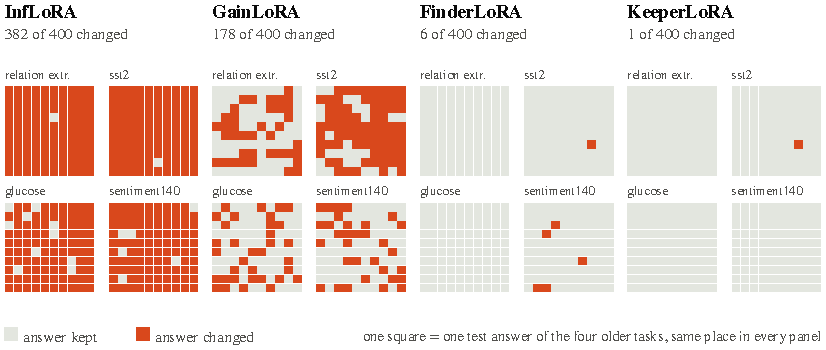
\includegraphics[width=\linewidth]{figures/answer_grid}
  \caption{Every square is one test answer. Five tasks without definitions, \AudFullEpochs{}
  epochs per task, seed 42: the \AudFullCompared{} test answers of the four older tasks, right
  after their task was learned against after the last task; a square has the same place in every
  panel. InfLoRA changes \AudFullInfloraChanged{} of the \AudFullCompared{} answers, GainLoRA
  \AudFullGainloraChanged{}, \recog{} \AudFullOursRidgeChanged{} and \handicap{}
  \AudFullOursHandicapChanged{}.}
  \label{fig:answergrid}
\end{figure}

\begin{figure}[t]
  \centering
  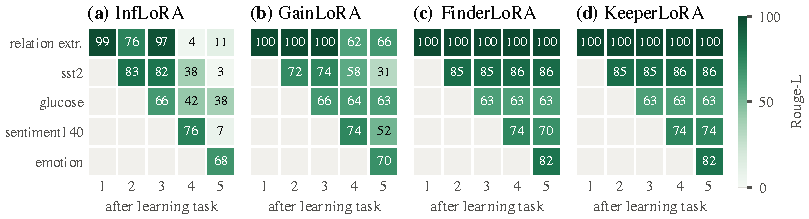
\includegraphics[width=\linewidth]{figures/stage_heatmap}
  \caption{The score of each task (rows) after each later task has been learned (columns), for the
  runs of Figure~\ref{fig:answergrid}; Rouge-L of the re-test (all reference answers), rounded. A
  row that keeps its colour is a task that is not forgotten: with InfLoRA and GainLoRA most rows of
  older tasks fade, with \recog{} and \handicap{} they stay.}
  \label{fig:stageheat}
\end{figure}


\paragraph{The control: the same methods with their definitions.} The loss of the published methods could come from the missing definition or from \AudFullEpochs{} epochs on this smaller model. Both were run with \AudFullEpochs{} epochs and the definitions left in; the definition is the only difference (Table~\ref{tab:fulldefinitions}).
Line fixed before the run, for each method: ``the instruction was what kept the answers'' if, with definitions, forgetting is at most half of its value without and at most half as many answers change; ``it was not the instruction'' if forgetting with definitions is at least 80\% of that without. Verdict: the first holds for both. GainLoRA forgets \AudFullDefOriginalGainloraFT{} points with definitions against \AudFullGainloraFT{} without, InfLoRA \AudFullDefOriginalInfloraFT{} against \AudFullInfloraFT{} (answers changed: Table~\ref{tab:fulldefinitions}). \recog{} and \handicap{}, which never read the definition, forget about one point or less.
With definitions and \AudFullEpochs{} epochs the two end below \cert{} and \recog{} with definitions and 10 epochs (Table~\ref{tab:fullwordings}, Appendix~\ref{app:noinstmore}; Section~\ref{sec:exampleroutes}); we did not train our adapters for \AudFullEpochs{} epochs with definitions. Under the heavy rewording they end lower still, with many more changed answers.
The guesses were right for InfLoRA and for the forgetting of GainLoRA; GainLoRA learned less than guessed (\AudFullDefOriginalGainloraLearned{} right after learning, against 79 to 84), and we had thought it more likely than not to end above our 10-epoch score, which it did not. One seed and five tasks. Figure~\ref{fig:learnkeep} puts the runs with and without definitions side by side.

\begin{figure}[t]
  \centering
  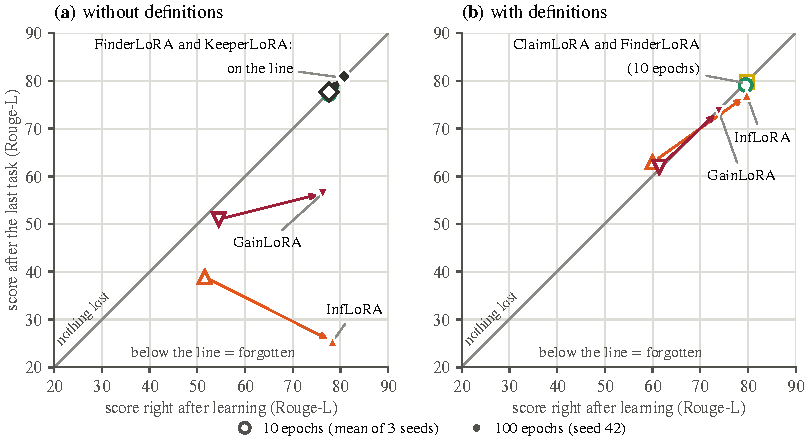
\includegraphics[width=\linewidth]{figures/learn_keep}
  \caption{Learned against kept, five tasks. A point is a method: its mean score right after
  learning ($x$) and after the last task ($y$). On the diagonal nothing is lost; the distance below
  it is what was forgotten. Hollow: 10 epochs (mean of three seeds); filled: \AudFullEpochs{} epochs
  (seed 42); an arrow goes from 10 to \AudFullEpochs{} epochs. (a)~Without definitions the two
  published methods learn more with more epochs and fall further below the diagonal; \recog{} and
  \handicap{} stay on it. (b)~With definitions the published methods stay near the diagonal (the
  control run); for our rules with definitions only 10-epoch runs exist.}
  \label{fig:learnkeep}
\end{figure}


\begin{table}[t]
  \caption{The definition as the only difference: the two published methods with \AudFullEpochs{} epochs per task, with and without definitions (five tasks, seed 42, re-test), and \recog{} and \handicap{} without definitions at the same epochs.}
  \label{tab:fulldefinitions}
  \centering
  {\footnotesize\setlength{\tabcolsep}{3pt}\begin{tabular}{p{1.9in}lrrrr}
    \toprule
    Method (seed 42, 100 epochs) & Definitions & \shortstack[r]{Score right\\after\\learning $\uparrow$} & \shortstack[r]{Final\\score $\uparrow$} & \shortstack[r]{Forgetting\\(points) $\downarrow$} & \shortstack[r]{Answers\\changed\\of \AudFullDefCompared{} $\downarrow$} \\
    \midrule
    InfLoRA & with & \AudFullDefOriginalInfloraLearned{} & \AudFullDefOriginalInfloraAP{} & \AudFullDefOriginalInfloraFT{} & \AudFullDefOriginalInfloraChanged{} \\
    InfLoRA & none & \AudFullInfloraLearned{} & \AudFullInfloraAP{} & \AudFullInfloraFT{} & \AudFullInfloraChanged{} \\
    \midrule
    GainLoRA & with & \AudFullDefOriginalGainloraLearned{} & \AudFullDefOriginalGainloraAP{} & \AudFullDefOriginalGainloraFT{} & \AudFullDefOriginalGainloraChanged{} \\
    GainLoRA & none & \AudFullGainloraLearned{} & \AudFullGainloraAP{} & \AudFullGainloraFT{} & \AudFullGainloraChanged{} \\
    \midrule
    \recog{} (ours) & none & \AudFullOursRidgeLearned{} & \AudFullOursRidgeAP{} & \AudFullOursRidgeFT{} & \AudFullOursRidgeChanged{} \\
    \handicap{} (ours) & none & \AudFullOursHandicapLearned{} & \AudFullOursHandicapAP{} & \AudFullOursHandicapFT{} & \AudFullOursHandicapChanged{} \\
    \bottomrule
\end{tabular}}

\end{table}

\begin{table}[t]
  \caption{The five tasks without definitions, seed 42, re-test: plain adapters behind \recog{} and \handicap{} and the two published methods, each with \AudFullEpochs{} epochs per task (the published number) and with 10. Columns as in Table~\ref{tab:noinstpublished}.}
  \label{tab:noinstfull}
  \centering
  {\footnotesize\setlength{\tabcolsep}{3pt}\begin{tabular}{p{1.95in}rrrr}
    \toprule
    Method, epochs (seed 42, no definition) & \shortstack[r]{Score right\\after\\learning $\uparrow$} & \shortstack[r]{Final\\score $\uparrow$} & \shortstack[r]{Forgetting\\(points) $\downarrow$} & \shortstack[r]{Answers\\changed\\of \AudFullCompared{} $\downarrow$} \\
    \midrule
    \recog{} (ours), 100 epochs & \AudFullOursRidgeLearned{} & \AudFullOursRidgeAP{} & \AudFullOursRidgeFT{} & \AudFullOursRidgeChanged{} \\
    \handicap{} (ours), 100 epochs & \AudFullOursHandicapLearned{} & \AudFullOursHandicapAP{} & \AudFullOursHandicapFT{} & \AudFullOursHandicapChanged{} \\
    \midrule
    InfLoRA, 100 epochs & \AudFullInfloraLearned{} & \AudFullInfloraAP{} & \AudFullInfloraFT{} & \AudFullInfloraChanged{} \\
    GainLoRA, 100 epochs & \AudFullGainloraLearned{} & \AudFullGainloraAP{} & \AudFullGainloraFT{} & \AudFullGainloraChanged{} \\
    \midrule
    InfLoRA, 10 epochs & \AudPubInfloraNoDefLearned{} & \AudPubInfloraNoDefAP{} & \AudPubInfloraNoDefFT{} & \AudPubInfloraNoDefChanged{} \\
    GainLoRA, 10 epochs & \AudPubGainloraNoDefLearned{} & \AudPubGainloraNoDefAP{} & \AudPubGainloraNoDefFT{} & \AudPubGainloraNoDefChanged{} \\
    \midrule
    \recog{} (ours), 10 epochs & \AudOursRidgeLearned{} & \AudOursRidgeAP{} & \AudOursRidgeFT{} & \AudOursRidgeChanged{} \\
    \handicap{} (ours), 10 epochs & \AudOursHandicapLearned{} & \AudOursHandicapAP{} & \AudOursHandicapFT{} & \AudOursHandicapChanged{} \\
    \bottomrule
\end{tabular}}

\end{table}

\begin{table}[t]
  \caption{The five tasks without definitions, means over \AudSeedsN{} seeds (42, 43, 44), re-test, 10 epochs. Final score with the lowest and highest seed; answers changed summed over the seeds. The route table of our rows is the same in every seed. Other columns as in Table~\ref{tab:noinstpublished}.}
  \label{tab:noinstseeds}
  \centering
  {\footnotesize\setlength{\tabcolsep}{2.5pt}\begin{tabular}{lrrrr}
    \toprule
    Method, no definition & \shortstack[r]{Score after\\learning $\uparrow$} & \shortstack[r]{Final\\score $\uparrow$} & \shortstack[r]{Forgetting\\(points) $\downarrow$} & \shortstack[r]{Answers changed\\of \AudSeedsCompared{} $\downarrow$} \\
    \midrule
    InfLoRA & \AudSeedsInfloraLearned{} & \AudSeedsInfloraAP{} {\scriptsize (\AudSeedsInfloraAPLow{}--\AudSeedsInfloraAPHigh{})} & \AudSeedsInfloraFT{} & \AudSeedsInfloraChanged{} \\
    GainLoRA & \AudSeedsGainloraLearned{} & \AudSeedsGainloraAP{} {\scriptsize (\AudSeedsGainloraAPLow{}--\AudSeedsGainloraAPHigh{})} & \AudSeedsGainloraFT{} & \AudSeedsGainloraChanged{} \\
    \midrule
    \plain{} & \AudSeedsPlainLearned{} & \AudSeedsPlainAP{} {\scriptsize (\AudSeedsPlainAPLow{}--\AudSeedsPlainAPHigh{})} & \AudSeedsPlainFT{} & \AudSeedsPlainChanged{} \\
    \centre{} & \AudSeedsCentreLearned{} & \AudSeedsCentreAP{} {\scriptsize (\AudSeedsCentreAPLow{}--\AudSeedsCentreAPHigh{})} & \AudSeedsCentreFT{} & \AudSeedsCentreChanged{} \\
    \recog{} (ours) & \AudSeedsRidgeLearned{} & \AudSeedsRidgeAP{} {\scriptsize (\AudSeedsRidgeAPLow{}--\AudSeedsRidgeAPHigh{})} & \AudSeedsRidgeFT{} & \AudSeedsRidgeChanged{} \\
    \handicap{} (ours) & \AudSeedsHandicapLearned{} & \AudSeedsHandicapAP{} {\scriptsize (\AudSeedsHandicapAPLow{}--\AudSeedsHandicapAPHigh{})} & \AudSeedsHandicapFT{} & \AudSeedsHandicapChanged{} \\
    own task (ceiling) & \AudSeedsOwnLearned{} & \AudSeedsOwnAP{} {\scriptsize (\AudSeedsOwnAPLow{}--\AudSeedsOwnAPHigh{})} & \AudSeedsOwnFT{} & \AudSeedsOwnChanged{} \\
    \bottomrule
\end{tabular}}

\end{table}

\begin{table}[t]
  \caption{Routes of the rules used in the GPU run, for the five-task sequence (500 test inputs, 400 of the first four tasks compared) and for the 15 SuperNI tasks: test inputs not at their own task after the last task; routes changed between arrival and the end, of those compared; audit $H/m$ and 95\% bound (Proposition~\ref{prop:audit}, averaged over all tasks of the sequence), where valid. The last row of each part sends every input to its own task.}
  \label{tab:routesgpu}
  \centering
  {\footnotesize\setlength{\tabcolsep}{3pt}\begin{tabular}{lrrrr}
    \toprule
    Rule & \shortstack[r]{Not sent\\to own task\\at the end $\downarrow$} & \shortstack[r]{Route\\changed $\downarrow$} & \shortstack[r]{Audit\\$H/m$, \%} & \shortstack[r]{95\% bound,\\\%} \\
    \midrule
    \multicolumn{5}{l}{\textit{five-task sequence}} \\
    \recog{} & \AudRouteFiveRidgeNotOwn{} of \AudRouteFiveRidgeN{} & \AudRouteFiveRidgeChanged{} of \AudRouteFiveRidgeCompared{} & \AudRouteFiveRidgeAuditEst{} & \AudRouteFiveRidgeAuditBound{} \\
    \handicap{}, $\nu = 2$ & \AudRouteFiveHandicapNotOwn{} of \AudRouteFiveHandicapN{} & \AudRouteFiveHandicapChanged{} of \AudRouteFiveHandicapCompared{} & -- & -- \\
    \recog{} with logistic regression & \AudRouteFiveJointNotOwn{} of \AudRouteFiveJointN{} & \AudRouteFiveJointChanged{} of \AudRouteFiveJointCompared{} & \AudRouteFiveJointAuditEst{} & \AudRouteFiveJointAuditBound{} \\
    every input to its own task (ceiling) & \AudRouteFiveOwnNotOwn{} of \AudRouteFiveOwnN{} & \AudRouteFiveOwnChanged{} of \AudRouteFiveOwnCompared{} & \AudRouteFiveOwnAuditEst{} & \AudRouteFiveOwnAuditBound{} \\
    \midrule
    \multicolumn{5}{l}{\textit{15 SuperNI tasks}} \\
    \recog{} & \AudRouteFifteenRidgeNotOwn{} of \AudRouteFifteenRidgeN{} & \AudRouteFifteenRidgeChanged{} of \AudRouteFifteenRidgeCompared{} & \AudRouteFifteenRidgeAuditEst{} & \AudRouteFifteenRidgeAuditBound{} \\
    \handicap{}, $\nu = 2$ & \AudRouteFifteenHandicapNotOwn{} of \AudRouteFifteenHandicapN{} & \AudRouteFifteenHandicapChanged{} of \AudRouteFifteenHandicapCompared{} & -- & -- \\
    \recog{} with logistic regression & \AudRouteFifteenJointNotOwn{} of \AudRouteFifteenJointN{} & \AudRouteFifteenJointChanged{} of \AudRouteFifteenJointCompared{} & \AudRouteFifteenJointAuditEst{} & \AudRouteFifteenJointAuditBound{} \\
    every input to its own task (ceiling) & \AudRouteFifteenOwnNotOwn{} of \AudRouteFifteenOwnN{} & \AudRouteFifteenOwnChanged{} of \AudRouteFifteenOwnCompared{} & \AudRouteFifteenOwnAuditEst{} & \AudRouteFifteenOwnAuditBound{} \\
    \bottomrule
\end{tabular}}

\end{table}

\paragraph{Fifteen tasks.} The same run on the 15 SuperNI tasks in their official order (no definitions; Table~\ref{tab:noinstfifteen}). The published methods were not run on fifteen tasks without definitions, so the line for that comparison cannot be read; retention can. Plain adapters behind \recog{} end at \AudFifteenNoDefRidgeAP{}, \AudFifteenNoDefRidgeBelowOwn{} points below the ceiling, with \AudFifteenNoDefRidgeChanged{} of \AudFifteenNoDefCompared{} changed answers; \handicap{} is similar. These are exactly the routes the route table changes (Lemma~\ref{lem:route}); with all adapters on the same adapters end at \AudFifteenNoDefPlainAP{} and every compared answer changes.
The guesses (score right after learning 39 to 43, final score within half a point, 8 to 20 changed answers) held. With definitions and the same epochs the published methods ended far lower, with many more changed answers (Table~\ref{tab:noinstfifteen}, Section~\ref{sec:fifteen}); they had learned less there, so that gap is partly learning. Our score right after learning is the same without definitions as with them (\AudFifteenNoDefOwnLearned{} and \AudFifteenDefCertLearned{}) by chance; the single tasks differ. These are the 15 tasks on which \recog{} was chosen. Figure~\ref{fig:routematrix} shows where the test inputs are sent after the last task.

\begin{figure}[t]
  \centering
  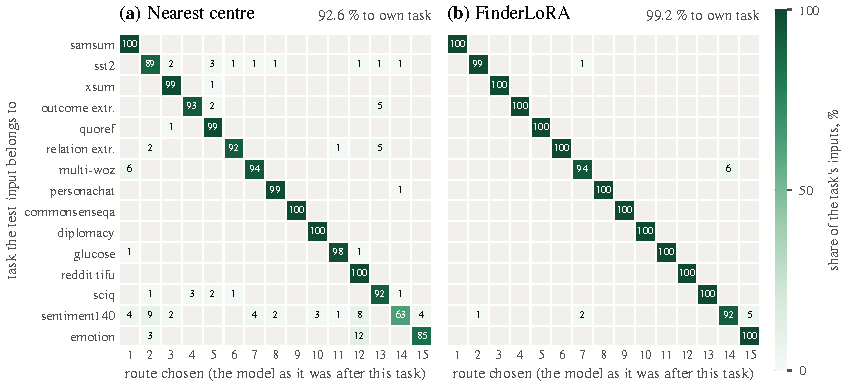
\includegraphics[width=\linewidth]{figures/route_matrix}
  \caption{Where the switch sends the test inputs: fifteen tasks without definitions, after the
  last task (seed 42). Rows: the task an input belongs to; columns: the route it gets; a cell is
  the share of the task's test inputs in per cent (shown from 1\,\%). (a)~The nearest centre sends
  \AudFifteenNoDefCentreRight{}\,\% of the inputs to their own task, (b)~\recog{}
  \AudFifteenNoDefRidgeRight{}\,\%.}
  \label{fig:routematrix}
\end{figure}


\begin{table}[t]
  \caption{The 15 SuperNI tasks without definitions, seed 42, 10 epochs, re-test: the same plain adapters under each rule; columns as in Table~\ref{tab:noinstfull}, last column the share at the own task after the last task. The three bottom rows are the run with definitions of Section~\ref{sec:fifteen}, for reference.}
  \label{tab:noinstfifteen}
  \centering
  {\footnotesize\setlength{\tabcolsep}{3pt}\begin{tabular}{p{1.75in}rrrrr}
    \toprule
    Method (seed 42, 15 tasks) & \shortstack[r]{Score right\\after\\learning $\uparrow$} & \shortstack[r]{Final\\score $\uparrow$} & \shortstack[r]{Forgetting\\(points) $\downarrow$} & \shortstack[r]{Answers\\changed\\of \AudFifteenNoDefCompared{} $\downarrow$} & \shortstack[r]{Sent to own\\task, \% $\uparrow$} \\
    \midrule
    \plain{} & \AudFifteenNoDefPlainLearned{} & \AudFifteenNoDefPlainAP{} & \AudFifteenNoDefPlainFT{} & \AudFifteenNoDefPlainChanged{} & \AudFifteenNoDefPlainRight{} \\
    \centre{} & \AudFifteenNoDefCentreLearned{} & \AudFifteenNoDefCentreAP{} & \AudFifteenNoDefCentreFT{} & \AudFifteenNoDefCentreChanged{} & \AudFifteenNoDefCentreRight{} \\
    \recog{} (ours) & \AudFifteenNoDefRidgeLearned{} & \AudFifteenNoDefRidgeAP{} & \AudFifteenNoDefRidgeFT{} & \AudFifteenNoDefRidgeChanged{} & \AudFifteenNoDefRidgeRight{} \\
    \handicap{} (ours) & \AudFifteenNoDefHandicapLearned{} & \AudFifteenNoDefHandicapAP{} & \AudFifteenNoDefHandicapFT{} & \AudFifteenNoDefHandicapChanged{} & \AudFifteenNoDefHandicapRight{} \\
    every input to its own task (ceiling) & \AudFifteenNoDefOwnLearned{} & \AudFifteenNoDefOwnAP{} & \AudFifteenNoDefOwnFT{} & \AudFifteenNoDefOwnChanged{} & \AudFifteenNoDefOwnRight{} \\
    \midrule
    \cert{}, with definitions & \AudFifteenDefCertLearned{} & \AudFifteenDefCertAP{} & \AudFifteenDefCertFT{} & \AudFifteenDefCertChanged{} & \AudFifteenDefCertRight{} \\
    GainLoRA, with definitions & \AudFifteenDefGainloraLearned{} & \AudFifteenDefGainloraAP{} & \AudFifteenDefGainloraFT{} & \AudFifteenDefGainloraChanged{} & -- \\
    InfLoRA, with definitions & \AudFifteenDefInfloraLearned{} & \AudFifteenDefInfloraAP{} & \AudFifteenDefInfloraFT{} & \AudFifteenDefInfloraChanged{} & -- \\
    \bottomrule
\end{tabular}}

\end{table}

\paragraph{What the results without instructions show.}
\emph{Reached:}
\begin{itemize}
\item A recogniser that reads no instruction, blocks no task, stores one vector per task and one matrix, and is the same for every order of arrival: \AudDevLLamOneEnd{}\% of test inputs at their own task after 15 tasks (development data).
\item An audit and a bound in advance, proved (Proposition~\ref{prop:audit}, Theorem~\ref{thm:handicap}); the measured change was within them in every run (averages over tasks, one split each; on the fresh batches the split does not ensure exchangeability).
\item Three rules passed their lines on fresh tasks, among them \recog{}; it also passed on the second benchmark (\AudScaleLongThreeEnd{}\%, routes only) and gives \AudScaleAllHundredTwentyEnd{}\% with 120 tasks.
\item In one reduced setting, trained answers beat the two published methods without instructions, by the line fixed before (re-test against re-test), at 10 and at \AudFullEpochs{} epochs; at \AudFullEpochs{} epochs the published methods learn the tasks and the gap is forgetting, and the control says the instruction held their answers.
\end{itemize}
\emph{Not reached:}
\begin{itemize}
\item The published setting (a larger model; the full number of epochs for one seed only), and the published methods on more than five tasks without definitions (ours ran on fifteen, one seed).
\item The second benchmark with trained answers; a tight bound in advance.
\item The published methods with an oracle for the task, or with our recogniser in front of them.
\item The upper side of the conflict $\Omega$ (the error of the best classifier between two tasks), and inputs that occur in two tasks, which no method without instructions can do better than split.
\end{itemize}
Choices made after seeing numbers (the features, \handicap{} and its floor, the zone shapes) give development numbers; only the fresh batches and the GPU run were read once against lines written before.
